%%%%%%%%%%%%%%%%%%%%%%%%%%%%%%%%%%%%%%%%%%%%%%%%%%%%%%%%%%%%%%
%%%%			Project October
%%%%
%%%%%%%%%%%%%%%%%%%%%%%%%%%%%%%%%%%%%%%%%%%%%%%%%%%%%%%%%%%%%%




\documentclass[11pt,letterpaper]{article}
\usepackage[utf8]{inputenc}
\usepackage[letterpaper,includeheadfoot, top=0.5cm, bottom=3.0cm, right=2.0cm, left=2.0cm]{geometry}
\renewcommand{\familydefault}{\sfdefault}

\usepackage{graphicx}
\usepackage{color}
\usepackage{amsmath}
\usepackage{hyperref}
\usepackage{amssymb}
\usepackage{url}
\usepackage{fancyhdr}
\usepackage{hyperref}
\usepackage{subfig}
\usepackage{pdfpages}

\usepackage{listings} %Code
\lstset{language=C, tabsize=4,framexleftmargin=5mm,breaklines=true}

\begin{document}
%\begin{sf}

\newpage
\pagestyle{fancy}
\fancyhf{}
\fancyhead[L]{ 
\includegraphics[scale=0.3]{img/cwru-formal-logo-blue-no-tag.png} }
\vspace*{6cm}
\begin{center}
\Huge  {Project October}\\
\vspace{1cm}
\huge {Read news that you want to read}\\
\vspace{1cm}
\end{center}
%----------------- Names ------------------------
\vfill
\begin{flushright}
\begin{tabular}{ll}
Authors: & Rajesh Cherukuri, Tom Dooner, Mika Little, Brian Stack\\
Project: & Project October\\
Date: & \today
\end{tabular}
\end{flushright}

\newpage
\pagestyle{fancy}
\fancyhf{}

\fancyhead[L]{\small \rm \textit{\rightmark}} 
\fancyhead[R]{\small \rm \textbf{\thepage}}



\renewcommand{\sectionmark}[1]{\markright{\thesection.\ #1}}
\renewcommand{\headrulewidth}{0.5pt}
\renewcommand{\footrulewidth}{0.5pt}

% =============== Index ===============

\tableofcontents
\listoffigures

% =============== Section ===============
\newpage
\section{Abstract}

In modern news aggregation services, such as Reddit, Slashdot, Digg, and Hacker News, longtime members report noticing a marked decrease in quality of discourse as the services gain mainstream attention. This gradual but irreversible decline caused by the influx of new users has been dubbed Eternal September. The loss of the longtime members perpetuates the problem, and causes large numbers of excellent contributors to be disenchanted and out-of-place in their own community. We aim to engineer a service that uses technological principles to avoid this, thus improving the user experience and allowing a large community to benefit from thoughtful discourse and interesting articles. \\

\newpage

%----Everything else----%

\section{October: Hybrid Recommender System}

This section will discuss the combination of a collaborative and content-based filtering in the context of web-based recommender systems. In particular, we will be linking various news sources and user submitted sources. the resulting network of user-item relations and associated content features is converted into a unified mathematical model, which is applicable to our underlying neighbor-based prediction algorithm. By means of various experiments, we demonstrate the influence of supplementary users as well as item features on the prediction accuracy of October, our proposed hybrid recommender. In order to decrease system runtime and to reveal latent user and item relations, we factorize our hybrid model via singular value decomposition (SVD).\\

\subsection{Background}

Due to the enormous amount of information available online, the need for highly developed personalization and filtering systems is growing permanently. Recommender systems constitute a specific type of information filtering that attempt to present items according the interests expressed by a user \cite{1}. Most web recommenders are employed for e-commerce applications or customer adapted websites, which assist users in decision making by providing personalized information \cite{5}.

In general, there exist two basic types of recommendation techniques, namely content-based filtering and collaborative filtering. Whereas content-based filtering methods examine items previously favored by the actual user \cite{7}, collaborative filtering techniques compute recommendations based on the information about similar items or users \cite{10}. In our work we combine both strategies into one hybrid approach \cite{3}, which utilizes supplementary content features in order to improve the prediction accuracy of traditional collaborative filtering \cite{6, 11}.

For the development and evaluation of our proposed hybrid recommender system (also referred to as October), we make use of various news outlets and user recommendations, importing them into a graph database. Both corpora are joined in a unified mathematical model, which describes the complex network of interdependencies. Our model is easy to extend and enables us to extract latent user/item relations by means of matrix factorization.

\subsection{Data Normalization}
When we compare the items of our Freebase rating matrix with entries of our generated feature matrices, we directly notice that both exhibit a unlikely range of values. Whereas article ratings are driven by number of "likes" (typically capped at about 250 for significance), content features are binary. Consequently, the original rating matrix $(R\in \{0,...,5\}^{m\times n})$ and user/item features matrices $(U\in \{0,1\}^{u\times y};I\in\{0,1\}^{x\times i})$ needs to be normalized differently.

\subsubsection{Subtractive Normalization}

Generally user-item ratings exhibit different kinds of global effects \cite{2, 4}. For instance, some users always tend to give higher ratings on items than other users, as well as some items at an average receive more positive user feedback than other items. In order to compute accurate rating predictions these global effect need to be removed form our data \cite{12}.

Usually a weighted combination of overall-, user- and item-average rating values ($\bar{r},\bar{r_u} \& \bar{r_i}$) is subtracted from the original entries ($r_{ui}$) to remove individual user preferences as well as item popularity effects \cite{10, 6, 8}:

$$\widetilde{r_{ui}} = r_{ui} - \alpha\bar{r} - \beta\bar{r_u} - \gamma\bar{r_i}$$

The parameters $\alpha$, $\beta$, and $\gamma$ determine the influence of the observed effects on the final normalization result. We make use of the least square estimation to automatically learn all normalization parameters \cite{4,12}.

\subsubsection{Multiplicative Normalization}

Since the entries of our generated feature matrices are either 0 or 1, all average values equal 1 ($\bar{r},\bar{r_u},\bar{r_i} = 1$). In case of subtractive normalization, the feature values would just be shifted instead of being regularized. Therefore we make use of multiplicative normalization, which regularizes all entries within a feature matrix F according to their respective row and column lengths:

$$ \widetilde{F} = M\cdot F\cdot N $$

where the diagonals of the matrices M and N contain the specific row and column multipliers:

$$ M_{xx} = \frac{1}{\sqrt{\sum_n F_{xn}}} \texttt{ and } N_{yy} = \frac{1}{\sqrt{\sum_m F_{my}}}$$

Note that all off-diagonal entries within the multiplication matrices are zero, and do not affect the normalization.

\subsection{Feature Combination}

We can combine the original rating matrix R and our retried user and item feature matrices ($U$ and $I$) are combined in a unified model:

$$ H_{m\times n} = \begin{bmatrix} R_{u\times i} & U_{u\times y}\cdot w_2 \\ I_{x\times i}\cdot w_1 & 0_{x\times y} \end{bmatrix} \texttt{ with } \begin{pmatrix} m = u + x \\ n = i + y \end{pmatrix}$$

Note that we need to fill our extended matrix with zeros to preserve the original rectangular shape. Moreover we have to keep in mind that the dimensions of the supplementary feature matrices have to fit our original rating matrix. Needless to say the respective user or rather item entries need to conform as well. Equation 4 reveals that the retrieved user and item features are assigned additional weights ($w_1$ and $w_2$ respectively). By means of these weights we can directly control the influence of the individual features on the final rating estimate. Our purpose is to identify those features and appropriate weights, which can improve the prediction accuracy of our hybrid recommender system. From here on, we assume the hybrid model H merely holds normalized rating and feature information.

\subsection{Matrix Factorization}

Typically matrix factorization techniques are used to reduce the dimension of the item space and/or to retrieve the latent relations between items of the observed dataset [9,4]. In our work we want to investigate the sophisticated \textit{Singular Value Decomposition (SVD)} approach, which factorizes our inflated rating matrix H into three low-dimensional matrices containing the left-singular vectors (V), the singular values (S), and right-singular vectors (W) respectively. In case of a reduction to dimension K, we can say the product of the resulting matrices is a rank-k approximation of our extended matrix $H_{m\times n}$:

$$H_k = V_{m\times k}\cdot S_{k\times k}\cdot {W_{k\times n}}^T$$

The prediction accuracy of our designed hybrid recommender system strongly depends on the parameter k, which we will discuss later.

\subsection{Rating Prediction}

Our generated matrices V, S and W can be utilized for the rating prediction step in several different ways \cite{9}. Probably the most straightforward method to estimate an unknown user-item rating ($r_{ui}$) is to simply multiple the according singular vectors and singular value (pure SVD approach):

$$ \hat{r_{ui}} = [VS^{0.5}]_u \cdot [S^{0.5}W^T]_i$$

But in our actual approach (HYB-SVD-KNN) we consider the compound matrices $ X = [VS^{0.5}]$ and $Y = [S^{0.5}W^T]$ as separate user and item concepts, which can be employed for user-oriented or rather item-oriented collaborative filtering. In case of item-oriented collaborative filtering, missing user-item ratings are calculated based on known ratings given by the same user on similar items \cite{10,8}:

$$\hat{r_{ui}} = \frac{\sum_{j\subset ratedItems(u)} s_{ij}\cdot r{uj}}{\sum_{j\in ratedItems(u)} |s_{ij}|}$$

where $s_{ij}$ represents the Cosine similarity of the according item vectors:

$$s_{ij} = \frac{Y_i\cdot Y_j}{||Y_i|| \cdot ||Y_j||}$$

In general, the prediction accuracy of a collaborative filtering system depends on the employed similarity measure as well as the number of examined neighborhood users/items that are involved in rating estimation \cite{12}. Therefore, we are going to scrutinize the influence of the neighborhood size in the following section.


\subsection{Evaluation}

As mentioned earlier, the prediction accuracy of our developed hybrid recommender depends on several different parameters, like neighborhood size, data dimension, utilized features and so on. This section will investigate the behavior of our system under certain conditions. We will be using the well known Root Mean Squared Error (metric used in the Netflix Prize Competition): $RMSE(O,P) = \sqrt{\frac{\sum_{i=1}^{n} (O_{i} - P_{i})^{2}}{n}}$ (where $O$ and $P$ are vectors of observed and predicted values respectively). RMSE will compute how close the estimates are to the values actually observed.\\

Finally, we are going to compare the overall performance of October with other implementation variants, at which prediction accuracy as well as computational effort are scrutinized.

\subsubsection{Neighborhood Size}

In general there exist two basic implementation variants of the KNN-algorithm, namely user- and item-oriented collaborative filtering. Whereas user-oriented techniques just consider like-minded users to predict unknown ratings, item-oriented methods utilize similar items \cite{10,13}. However both collaborative filtering variants employ the same underlying mathematical approach, in which the current examined user/item rating is estimated based on the $k$-nearest neighbors.

Obviously our item-oriented approach performs much better than the user-oriented implementation, which agrees with the general observations about collaborative filtering systems that can be found in most literature \cite{8, 2}, and might be explained by the fact that individuals are more familiar with the items previously preferred than with potential like-minded users.

The comparison furthermore reveals that a relatively small neighborhood produces imprecise rating estimates, which is due to the fact that the considered users or rather items do not contain sufficient information to make reliable predictions. However, in case of a comparatively large neighborhood it might happen that too many users or items with very low similarities are taken into account \cite{4, 6}.

For our further analysis we will make use of the optimum neighborhood size determined for user-oriented and item-oriented collaborative filtering respectively ($n = 25/70$).

\subsubsection{Data Dimension}

The prediction accuracy of our hybrid recommender system furthermore depends on the dimension k of the decomposed matrices (V, S and W; see Eq.(5)) \cite{10, 4}. Whereas relatively short singular vectors do not have enough explanatory power to differentiate the appropriate users or items, comparatively long vectors might lead to over-fitting.\\

As before, the item-oriented implementation produces better prediction results than the user-oriented counterpart. The displayed mixed approach of our SVD-KNN algorithm can be described as a weighted combination ($70$/$30$ ratio o user/item oriented collaborative filtering estimates) of user-oriented and item-oriented prediction results. However, this method could only achieve considerable performance improvements when supplementary user or rather item features were taken into account.\\

According to the comparison of the individual methods and the combined method, the global minimum of our user-oriented as well as mixed collaborative filtering approach is reached at a dimension of k = 10. For further studies on our item-oriented approach we set k = 20, because the dimension of the global minimum is quite high (k = 40) and produces an unsatisfactory system runtime.

\subsubsection{Feature Weights}

Besides analyzing the influence of neighborhood size and data dimension, we additionally investigate the effect of the retrieved user- and item-features on the prediction accuracy of our design hybrid recommender. As mentioned earlier, the contribution of the single user and item features is regulated by weights. We can show the behavior of October under the influence of various weighted features, employing the optimal parameter settings determined previously ($n = \frac{25}{70}$ and $k=\frac{10}{20}$). \\

All user and item features are selected based on their matrix fill-rate, where as only feature matrices with a low sparsity ($\leq 99\% $) are considered for rating prediction. This is due to the fact that sparse feature matrices do not increase the explanatory power of our original rating matrix R. In our research, we investigate public user profile information of the examined Freebase users as well as geolocation, date, and category of the appropriate media.\\

The performance improvement made by the examined media features is much higher than by the considered user features. In particular, the Media-\{Age-Country\} feature produced surpassing prediction results. But the highest prediction accuracy could be achieved by the combination of both individual user and item features. This can also be evidenced by taking the item- or user-oriented collaborative filtering methods using similar features, which still show that October outperforms them to provide lower RMSE values across the board.

Besides contrasting the prediction accuracy of these algorithms, we furthermore want to scrutinize their runtime. We can show a juxtaposition of the individual rating prediction methods, where the computational effort is presented on a logarithmic scale. Note that the algorithm runtime is directly dependent on the available processing power.

In general, the performance and runtime of recommender systems are in competition and have a mutual influence on each other. For this reason we need to treat a recommender with all its factors as a whole. According to performance benchmarks, our proposed hybrid recommender October is superior in terms of prediction accuracy. Although the pure SVD approach shows the lowest computational effort, our hybrid method is about four times faster than traditional KNN collaborative filtering. On that account we believe that October is practical to media recommendation for real-world users.

\subsection{Algorithm}

% ---To be added--------------------

% ----------------------------------



% ============= References ==============
\newpage
\newpage
\begin{thebibliography}{13}	
  \bibitem{1} Gediminas Adomavicius , Alexander Tuzhilin, \textit{Toward the Next Generation of Recommender Systems: A Survey of the State-of-the-Art and Possible Extensions}, IEEE Transactions on Knowledge and Data Engineering, v.17 n.6, p.734-749, June 2005  [doi>10.1109/TKDE.2005.99]

  \bibitem{2} Robert M. Bell , Yehuda Koren, \textit{Scalable Collaborative Filtering with Jointly Derived Neighborhood Interpolation Weights, Proceedings of the 2007 Seventh IEEE International Conference on Data Mining}, p.43-52, October 28-31, 2007  [doi>10.1109/ICDM.2007.90]

  \bibitem{3} R. D. Burke. Hybrid web recommender systems. In P. Brusilovsky, A. Kobsa, and W. Nejdl, editors, \textit{The Adaptive Web, Methods and Strategies of Web Personalization}, volume 4321 of Lecture Notes in Computer Science, pages 377--408. Springer, 2007.

  \bibitem{4} Yehuda Koren, \textit{Factorization meets the neighborhood: a multifaceted collaborative filtering model}, Proceeding of the 14th ACM SIGKDD international conference on Knowledge discovery and data mining, August 24-27, 2008, Las Vegas, Nevada, USA  [doi>10.1145/1401890.1401944]

  \bibitem{5} Greg Linden , Brent Smith , Jeremy York, \textit{Amazon.com Recommendations: Item-to-Item Collaborative Filtering}, IEEE Internet Computing, v.7 n.1, p.76-80, January 2003  [doi>10.1109/MIC.2003.1167344]

  \bibitem{6} Prem Melville , Raymod J. Mooney , Ramadass Nagarajan, \textit{Content-boosted collaborative filtering for improved recommendations, Eighteenth national conference on Artificial intelligence}, p.187-192, July 28-August 01, 2002, Edmonton, Alberta, Canada

  \bibitem{7} M. J. Pazzani and D. Billsus. \textit{Content-based recommendation systems}. In P. Brusilovsky, A. Kobsa, and W. Nejdl, editors, The Adaptive Web, volume 4321 of Lecture Notes in Computer Science, chapter 10, pages 325--341. Springer-Verlag, Berlin, Germany, May 2007.

  \bibitem{8} Badrul Sarwar , George Karypis , Joseph Konstan , John Reidl, \textit{Item-based collaborative filtering recommendation algorithms}, Proceedings of the 10th international conference on World Wide Web, p.285-295, May 01-05, 2001, Hong Kong, Hong Kong  [doi>10.1145/371920.372071]

  \bibitem{9} B. M. Sarwar, G. Karypis, J. A. Konstan, and J. T. Riedl. \textit{Application of dimensionality reduction in recommender system - a case study}. In In ACM WebKDD Workshop, 2000.

  \bibitem{10} J. B. Schafer, D. Frankowski, J. Herlocker, and S. Sen. \textit{Collaborative filtering recommender systems}. In P. Brusilovsky, A. Kobsa, and W. Nejdl, editors, The Adaptive Web, volume 4321 of Lecture Notes in Computer Science, chapter 9, pages 291--324. Springer-Verlag, Berlin, Germany, may 2007.

  \bibitem{11} David H. Stern , Ralf Herbrich , Thore Graepel, \textit{Matchbox: large scale online bayesian recommendations}, Proceedings of the 18th international conference on World wide web, April 20-24, 2009, Madrid, Spain  [doi>10.1145/1526709.1526725]

  \bibitem{12} A. Toescher, M. Jahrer, and R. Legenstein. \textit{Improved neighborhood-based algorithms for large-scale recommender systems}. In KDD '08: Proceeding of the 14th ACM SIGKDD international conference on Knowledge discovery and data mining, Graz, Austria, 2008. ACM.

  \bibitem{13} Jun Wang , Arjen P. de Vries , Marcel J. T. Reinders, \textit{Unifying user-based and item-based collaborative filtering approaches by similarity fusion}, Proceedings of the 29th annual international ACM SIGIR conference on Research and development in information retrieval, August 06-11, 2006, Seattle, Washington, USA  [doi>10.1145/1148170.1148257]
  
\end{thebibliography}

% ============= Database Schematic ==============
\begin{figure}
\centering
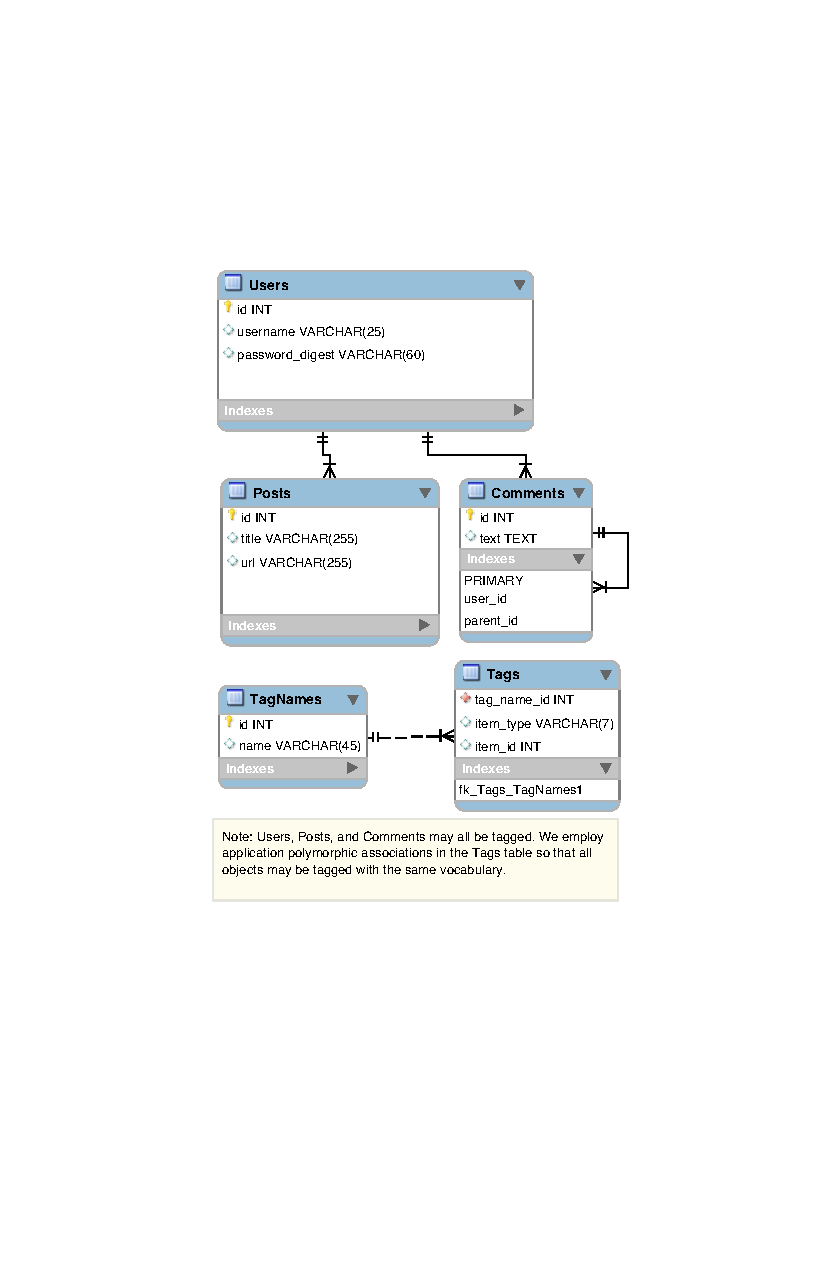
\includegraphics{db_diagram.pdf}
\caption{Frontend Database Relational Diagram}
\label{fig:database}
\end{figure}

% ============= FIN ==============
\end{document}

